\addchap{Symbols and Names}
\addsec*{Pentagrams}
\subsection*{Divine Names}
\begin{center}
\large
\begin{tabular}{ r | lr | l }
  Element & Name & & Pronunciation \\
  \hline
  Spirit (Active) & A H I H & \cjRL{'hyh} & Eheieh \\
  Spirit (Passive) & A G L A & \cjRL{'gl'} & Agla \\
  Fire & A L H I M & \cjRL{'lhym} & Elohim \\
  Water & A L & \cjRL{'l} & El \\
  Air & I H V H & \cjRL{yhwh} & Ye-ho-wau \\
  Earth & A D N I & \cjRL{'dny} & Adonai \\
\end{tabular}
\end{center}
\footnotetext[99]{Images thanks to Thelemapedia \textemdash{} released under GNU Free Documentation License v1.2}
\subsection*{Invoking}
\begin{center}
\makebox[\textwidth]{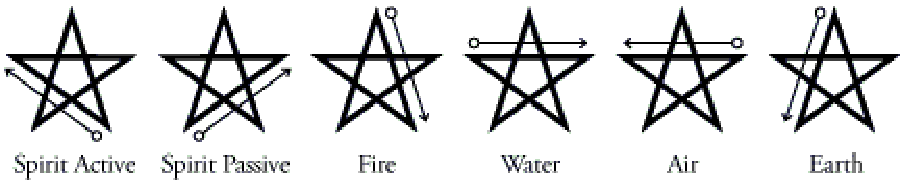
\includegraphics[scale=.55,keepaspectratio]{images/invokingpentagrams}}
\end{center}
\subsection*{Banishing}
\begin{center}
\makebox[\textwidth]{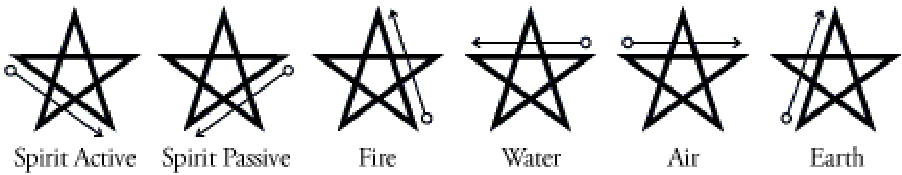
\includegraphics[scale=.55,keepaspectratio]{images/banishingpentagrams}}
\end{center}
\addsec*{Liber V vel Reguli\footnote{Invoking Averse Pentagrams.\footnotemark}\footnotetext{I have found that averse pentagram forms may be adapted for banishing in my rituals; start at the arrow heads and go towards the circles, similar to the invoking/banishing aright pentagrams.}}
\begin{center}
\makebox[\textwidth]{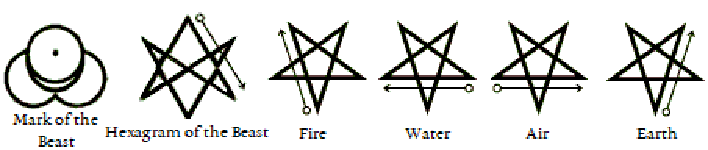
\includegraphics[scale=.72,keepaspectratio]{images/averse}}
\end{center}
\addsec*{Elemental Hexagrams}
\subsection*{Invoking}
\begin{center}
\makebox[\textwidth]{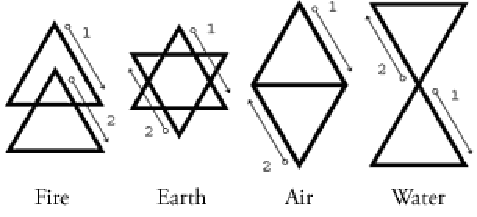
\includegraphics[scale=.70,keepaspectratio]{images/invokinghexagrams}}
\end{center}
\subsection*{Banishing}
\begin{center}
\makebox[\textwidth]{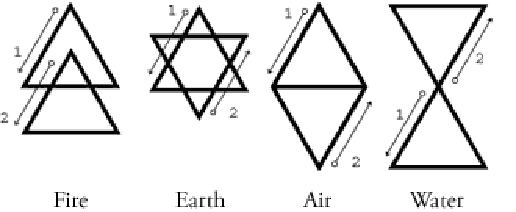
\includegraphics[scale=.70,keepaspectratio]{images/banishinghexagrams}}
\end{center}

The Unicursal Hexagram may be used for invoking and banishing various forces. See Frater David R Jones' \textit{On the Formulae of the Unicursal Hexagram} for an explanation.

There are several planetary hexagrams and astrological sigils omitted from here, used in the Greater Ritual of the Hexagram in particular.
